\chapter{Fundamentos Teóricos e Conceptos Previos}

En este capítulo se exponen los fundamentos teóricos en los que se basa el proyecto o que se
utilizan en él.
Normalmente cada proyecto trata de una temática, de la que hay una serie de conocimientos
teóricos relacionados y que deben incluirse en la memoria del proyecto, para aportarle el carácter
científico que conlleva todo trabajo académico.
Se requiere una explicación detallada de todo lo necesario, para dar una visión profunda de lo
que debe conocerse para afrontar la realización del proyecto. Por una parte sirve como exposición
de los elementos científicos en los que se basa el proyecto, pero a la vez, como explicación de lo
que se ha estudiado para la elaboración del mismo.

\section{Análise do comportamento}
	
	É un dos campos de investigación mas activos hoxe en día. A idea principal 
	deste tipo de sistemas é a de detectar calquera acción levada a cabo polos 
	obxectos involucrados. Un obxecto é calquera cousa que debe ser seguida, polo
	que dependendo do tipo de problema estes obxectos poden ser dunha natureza ou doutra.
	Por outra parte, o tipo de accións depende do que o sistema trate de detectar, xa poden
	ser comportamentos individuais( camiñar, correr, loitar...) ou grupais (reunirse, 
	abandonar un grupo de persoas...).
	
	Á súa vez os sistemas de análise de comportamento poder dividirse en tres 
	técnicas diferentes\cite{brais-thesis}:
	
	\begin{itemize}
	
		\item{\textbf{Detección:}} A partires de unha secuencia de vídeo como entrada obtén os 
		distintos obxectos que aparecen en cada fotograma da escena. Para este fin empréganse
		técnicas de visión por computador.
		
		%Aqui podríame extender falando da Substracción de Fondo, o Fluxo Óptico e os Sistemas de alto Nivel
		
		\item{\textbf{Seguimento:}} A partires da información obtida na detección, asígnanselle 
		identificadores a cada obxecto detectado no vídeo, agrupando se procede distintos
		obxectos baixo o mesmo identificador, se se considera que estes obxectos forman
		parte de un grupo ou unha mesma detección.
		
		% Aquí podría falar das aproximacións por apariencia, filtro de Kalman, filtro de Partículas ..
		
		\item{\textbf{Análise do comportamento de Alto Nivel:}} A partires da información obtida nos 
		dous pasos anteriores pódese catalogar o comportamento de cada detección empregando
		técnicas de recoñecemento de patróns.
	
	\end{itemize}	
	
	Os resultados mais destacables destas técnicas cos que a aplicación terá que traballar serán:
	\begin{itemize}
		\item A lista de obxectos detectados para cada un dos fotogramas e a súa posición neles
		\item A traxectoria de cada un dos obxectos detectados
		\item O grao de anormalidade da traxectoria seguida por un obxecto en cada un dos fotogramas
		\item A velocidade de un obxecto determinado.
	\end{itemize}
	
	\subsection{OpenCV}
		OpenCV é unha biblioteca libre de visión artificial escrita en código C/C++ optimizado.
		Dende a súa aparición publicada por Intel en Xaneiro de 1999, empregouse en infinidade 
		de proxectos. Tanto para detección de movemento como para aplicativos de control de procesos
		que requiren recoñecemento de obxectos.
		
		OpenCV é multiplataforma, existindo versión para GNU/Linux, Mac OS X e Windows. Contén mais 
		de 500 funcións que abarcan unha ampla gama de áreas como o proceso de visión, recoñecemento
		de obxectos (tamén recoñecemento facial), calibrado de cámaras, realidade aumentada e visión
		robótica.
		
		A aplicación a desenvolver ten que garantir a compatibilidade cos algoritmos creados sobre
		OpenCV. Isto farase definindo unha interface de liña de comando e un formato de ficheiro XML
		(Extensible Markup Language) no que as aplicación de recoñecemento deben escribir os datos da
		súa análise.
		
\section{Extensible Markup Language (XML)}
	XML é unha linguaxe de marcas desenvolvida polo World Wide Web Consortium (W3C) e empregado
	para almacenar datos de forma clara e lexible. Permite definir a gramática de linguaxes 
	específicas para estruturar así grandes documentos.
	XML é especialmente útil para comunicar varias aplicacións que traballan en tecnoloxías 
	diferentes, xa que grazas á súa simplicidade é extremadamente sinxelo integrar os datos.
	
	Os documentos XML seguen una estrutura xerárquica baseada en etiquetas(tag's) e atributos,
	que se poden definir nunha Definición de Tipo de Documento ou DTD. \cite{dtd-web-page}
	
	Cando un documento en formato XML segue as directrices definidas no ficheiro DTD asociado,
	dise que este ficheiro esta ben formado(well formed en ingles), e para validar iso empregarase
	na elaboración do traballo algún avaliador de XML en liña como por exemplo o da W3Chools.\cite{xml-validator}
	
\section{Programación Web}

	A programación web de Aplicacións de carácter empresarial require do coñecemento da rede, ademais
	do de unha serie de ferramentas e estratexias para chegar a un deseño sostible e de calidade.
	
	A arquitectura clásica das aplicacións web pódese ver no gráfico \ref{fig:ArquitecturaAppWeb}
	
	\begin{figure}[htp]
	\begin{center}
		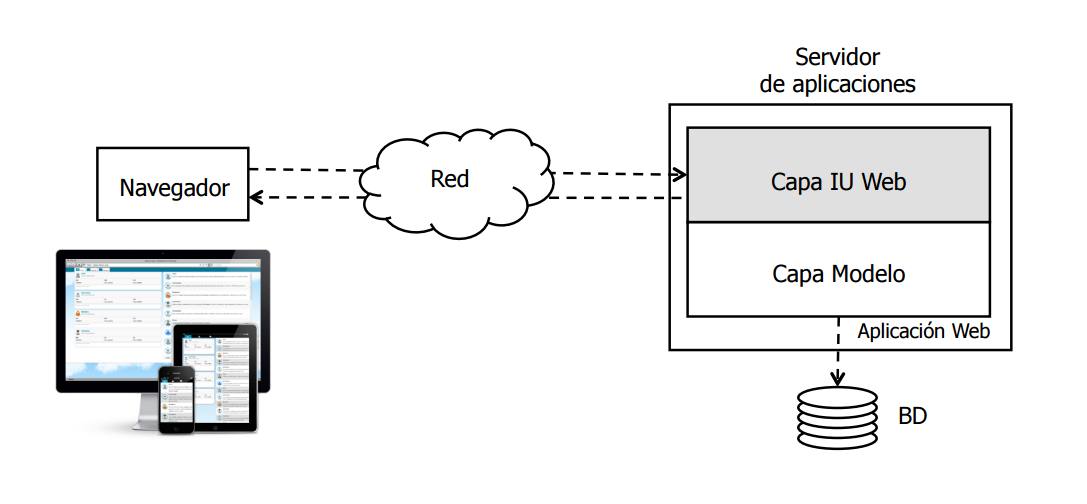
\includegraphics[scale=0.35]{figures/ArquitecturaAppWeb.png}
		\caption{Clásica arquitectura dunha aplicación web empresarial}
	\label{fig:ArquitecturaAppWeb}
	\end{center}
	\end{figure}


	Os puntos claves da programación clave son:
	
	\subsection {Desenvolvemento Áxil}
		Para reducir custos e poder proporcionar solucións rápidas é preciso que as 
		aplicacións web's de caracter empresarial se leven a cabo en pouco tempo e con
		bos principios de enxeñaría.
	
	\subsection{Soporte para transaccións}
		Unha transacción nun Sistema Xestor de Base de Datos (SGBD) é un conxunto de ordes que
		se executan formando unha unidade de traballo, de forma invisible e atómica. As transaccións
		cobran gran importancia nas aplicacións webs debido á inestabilidade da rede, e á concorrencia
		dos distintos clientes conectados.
	
	\subsection{Object-Relational Mapping (ORM)}
		Os mapeado obxecto-relación, é unha tecnica de programación para converter datos de unha 
		linguaxe Orientada a Obxectos (OO) a datos de un sistema relacional no que son persistidos 
		e viceversa. Dispoñer de un mapeador obxecto-relacional ben integrado coa tecnoloxía a 
		empregar minimiza drasticamente o tempo preciso para o desenvolvemento das funcionalidades.
	
	\subsection{Xestión de Layout}
		Tamén resulta moi practico dispoñer dunha linguaxe de prantilla que permitan xerar contido
		html dinamicamente. Algúns exemplos son o Sistema de Templates de Django, o Sistema JSP de Spring,
		a libraría Thymeleaf ou os compoñentes de ASP.NET. Todos eles axudan a xerar contido HTML de
		xeito sinxelo e escalable.
		
	\subsection{Outras cuestións da web}
		A maiores existe toda unha gama de outras funcionalidades que cobran importancia cando deseñamos
		e construímos unha web como o manexo de erros nos formularios, internacionalización (i18n), 
		visualización de grande cantidades de datos(en listas ou táboas), seguridade... 
  
  
\chapter{Análise de antecedentes e alternativas}
	Se trata de realizar un estudio de alternativas o “estado del arte” o un análisis comparativo
	de alternativas.

	Se exponen las diferentes alternativas que se han evaluado o que se consideran de interés, a
	lo realizado en el proyecto. Fundamentalmente se trata de otras herramientas existentes 
	que realizan algo similar, sean o no comerciales, o de prototipos de investigación relacionados,
	o de estudios que tratan aspectos similares.

	Buscar por internet produtos que fagan algo similar...